% Lines starting with a percent sign (%) are comments. LaTeX will
% not process those lines. Similarly, everything after a percent
% sign in a line is considered a comment. To produce a percent sign
% in the output, write \% (backslash followed by the percent sign).
% ==================================================================
% Usage instructions:
% ------------------------------------------------------------------
% The file is heavily commented so that you know what the various
% commands do. Feel free to remove any comments you don't need from
% your own copy. When redistributing the example thesis file, please
% retain all the comments for the benefit of other thesis writers!
% ==================================================================
% Compilation instructions:
% ------------------------------------------------------------------
% Use pdflatex to compile! Input images are expected as PDF files.
% Example compilation:
% ------------------------------------------------------------------
% > pdflatex thesis-example.tex
% > bibtex thesis-example
% > pdflatex thesis-example.tex
% > pdflatex thesis-example.tex
% ------------------------------------------------------------------
% You need to run pdflatex multiple times so that all the cross-references
% are fixed. pdflatex will tell you if you need to re-run it (a warning
% will be issued)
% ------------------------------------------------------------------
% Compilation has been tested to work in ukk.cs.hut.fi and kosh.hut.fi
% - if you have problems of missing .sty -files, then the local LaTeX
% environment does not have all the required packages installed.
% For example, when compiling in vipunen.hut.fi, you get an error that
% tikz.sty is missing - in this case you must either compile somewhere
% else, or you cannot use TikZ graphics in your thesis and must therefore
% remove or comment out the tikz package and all the tikz definitions.
% ------------------------------------------------------------------

% General information
% ==================================================================
% Package documentation:
%
% The comments often refer to package documentation. (Almost) all LaTeX
% packages have documentation accompanying them, so you can read the
% package documentation for further information. When a package 'xxx' is
% installed to your local LaTeX environment (the document compiles
% when you have \usepackage{xxx} and LaTeX does not complain), you can
% find the documentation somewhere in the local LaTeX texmf directory
% hierarchy. In ukk.cs.hut.fi, this is /usr/texlive/2008/texmf-dist,
% and the documentation for the titlesec package (for example) can be
% found at /usr/texlive/2008/texmf-dist/doc/latex/titlesec/titlesec.pdf.
% Most often the documentation is located as a PDF file in
% /usr/texlive/2008/texmf-dist/doc/latex/xxx, where xxx is the package name;
% however, documentation for TikZ is in
% /usr/texlive/2008/texmf-dist/doc/latex/generic/pgf/pgfmanual.pdf
% (this is because TikZ is a front-end for PGF, which is meant to be a
% generic portable graphics format for LaTeX).
% You can try to look for the package manual using the ``find'' shell
% command in Linux machines; the find databases are up-to-date at least
% in ukk.cs.hut.fi. Just type ``find xxx'', where xxx is the package
% name, and you should find a documentation file.
% Note that in some packages, the documentation is in the DVI file
% format. In this case, you can copy the DVI file to your home directory,
% and convert it to PDF with the dvipdfm command (or you can read the
% DVI file directly with a DVI viewer).
%
% If you can't find the documentation for a package, just try Googling
% for ``latex packagename''; most often you can get a direct link to the
% package manual in PDF format.
% ------------------------------------------------------------------


% Document class for the thesis is report
% ------------------------------------------------------------------
% You can change this but do so at your own risk - it may break other things.
% Note that the option pdftext is used for pdflatex; there is no
% pdflatex option.
% ------------------------------------------------------------------
\documentclass[12pt,a4paper,oneside,pdftex]{report}

% The input files (tex files) are encoded with the latin-1 encoding
% (ISO-8859-1 works). Change the latin1-option if you use UTF8
% (at some point LaTeX did not work with UTF8, but I'm not sure
% what the current situation is)
\usepackage[latin1]{inputenc}
% OT1 font encoding seems to work better than T1. Check the rendered
% PDF file to see if the fonts are encoded properly as vectors (instead
% of rendered bitmaps). You can do this by zooming very close to any letter
% - if the letter is shown pixelated, you should change this setting
% (try commenting out the entire line, for example).
\usepackage[OT1]{fontenc}
% The babel package provides hyphenating instructions for LaTeX. Give
% the languages you wish to use in your thesis as options to the babel
% package (as shown below). You can remove any language you are not
% going to use.
% Examples of valid language codes: english (or USenglish), british,
% finnish, swedish; and so on.
\usepackage[finnish,english]{babel}

% placeins allows for use of FloatBarrier, which helps with the layout of the
% results chapter
\usepackage{placeins}

% for mathstuff
\usepackage{amssymb}

% Font selection
% ------------------------------------------------------------------
% The default LaTeX font is a very good font for rendering your
% thesis. It is a very professional font, which will always be
% accepted.
% If you, however, wish to spicen up your thesis, you can try out
% these font variants by uncommenting one of the following lines
% (or by finding another font package). The fonts shown here are
% all fonts that you could use in your thesis (not too silly).
% Changing the font causes the layouts to shift a bit; you many
% need to manually adjust some layouts. Check the warning messages
% LaTeX gives you.
% ------------------------------------------------------------------
% To find another font, check out the font catalogue from
% http://www.tug.dk/FontCatalogue/mathfonts.html
% This link points to the list of fonts that support maths, but
% that's a fairly important point for master's theses.
% ------------------------------------------------------------------
% <rant>
% Remember, there is no excuse to use Comic Sans, ever, in any
% situation! (Well, maybe in speech bubbles in comics, but there
% are better options for those too)
% </rant>

% \usepackage{palatino}
% \usepackage{tgpagella}



% Optional packages
% ------------------------------------------------------------------
% Select those packages that you need for your thesis. You may delete
% or comment the rest.

% Natbib allows you to select the format of the bibliography references.
% The first example uses numbered citations:
\usepackage[square,sort&compress,numbers]{natbib}
% The second example uses author-year citations.
% If you use author-year citations, change the bibliography style (below);
% acm style does not work with author-year citations.
% Also, you should use \citet (cite in text) when you wish to refer
% to the author directly (\citet{blaablaa} said blaa blaa), and
% \citep when you wish to refer similarly than with numbered citations
% (It has been said that blaa blaa~\citep{blaablaa}).
% \usepackage[square]{natbib}

% The alltt package provides an all-teletype environment that acts
% like verbatim but you can use LaTeX commands in it. Uncomment if
% you want to use this environment.
% \usepackage{alltt}

% The eurosym package provides a euro symbol. Use with \euro{}
\usepackage{eurosym}

% Verbatim provides a standard teletype environment that renderes
% the text exactly as written in the tex file. Useful for code
% snippets (although you can also use the listings package to get
% automatic code formatting).
\usepackage{verbatim}

% The listing package provides automatic code formatting utilities
% so that you can copy-paste code examples and have them rendered
% nicely. See the package documentation for details.
% \usepackage{listings}

% The fancuvrb package provides fancier verbatim environments
% (you can, for example, put borders around the verbatim text area
% and so on). See package for details.
% \usepackage{fancyvrb}

% Supertabular provides a tabular environment that can span multiple
% pages.
%\usepackage{supertabular}
% Longtable provides a tabular environment that can span multiple
% pages. This is used in the example acronyms file.
\usepackage{longtable}

% The fancyhdr package allows you to set your the page headers
% manually, and allows you to add separator lines and so on.
% Check the package documentation.
% \usepackage{fancyhdr}

% Subfigure package allows you to use subfigures (i.e. many subfigures
% within one figure environment). These can have different labels and
% they are numbered automatically. Check the package documentation.
%\usepackage{subfigure}
\usepackage{subcaption}
% The titlesec package can be used to alter the look of the titles
% of sections, chapters, and so on. This example uses the ``medium''
% package option which sets the titles to a medium size, making them
% a bit smaller than what is the default. You can fine-tune the
% title fonts and sizes by using the package options. See the package
% documentation.
\usepackage[medium]{titlesec}

% The TikZ package allows you to create professional technical figures.
% The learning curve is quite steep, but it is definitely worth it if
% you wish to have really good-looking technical figures.
\usepackage{tikz}
% You also need to specify which TikZ libraries you use
\usetikzlibrary{positioning}
\usetikzlibrary{calc}
\usetikzlibrary{arrows}
\usetikzlibrary{decorations.pathmorphing,decorations.markings}
\usetikzlibrary{shapes}
\usetikzlibrary{patterns}



\usepackage{caption}
% The aalto-thesis package provides typesetting instructions for the
% standard master's thesis parts (abstracts, front page, and so on)
% Load this package second-to-last, just before the hyperref package.
% Options that you can use:
%   mydraft - renders the thesis in draft mode.
%             Do not use for the final version.
%   doublenumbering - [optional] number the first pages of the thesis
%                     with roman numerals (i, ii, iii, ...); and start
%                     arabic numbering (1, 2, 3, ...) only on the
%                     first page of the first chapter
%   twoinstructors  - changes the title of instructors to plural form
%   twosupervisors  - changes the title of supervisors to plural form
\usepackage[mydraft,twosupervisors]{aalto-thesis}
%\usepackage[mydraft,doublenumbering]{aalto-thesis}
%\usepackage{aalto-thesis}


% Hyperref
% ------------------------------------------------------------------
% Hyperref creates links from URLs, for references, and creates a
% TOC in the PDF file.
% This package must be the last one you include, because it has
% compatibility issues with many other packages and it fixes
% those issues when it is loaded.
\RequirePackage[pdftex]{hyperref}
% Setup hyperref so that links are clickable but do not look
% different
\hypersetup{colorlinks=false,raiselinks=false,breaklinks=true}
\hypersetup{pdfborder={0 0 0}}
\hypersetup{bookmarksnumbered=true}
% The following line suggests the PDF reader that it should show the
% first level of bookmarks opened in the hierarchical bookmark view.
\hypersetup{bookmarksopen=true,bookmarksopenlevel=1}
% Hyperref can also set up the PDF metadata fields. These are
% set a bit later on, after the thesis setup.


% Thesis setup
% ==================================================================
% Change these to fit your own thesis.
% \COMMAND always refers to the English version;
% \FCOMMAND refers to the Finnish version; and
% \SCOMMAND refers to the Swedish version.
% You may comment/remove those language variants that you do not use
% (but then you must not include the abstracts for that language)
% ------------------------------------------------------------------
% If you do not find the command for a text that is shown in the cover page or
% in the abstract texts, check the aalto-thesis.sty file and locate the text
% from there.
% All the texts are configured in language-specific blocks (lots of commands
% that look like this: \renewcommand{\ATCITY}{Espoo}.
% You can just fix the texts there. Just remember to check all the language
% variants you use (they are all there in the same place).
% ------------------------------------------------------------------
\newcommand{\TITLE}{Stream Processing on a Multicore DSP with Open Event Machine}
\newcommand{\FTITLE}{OpenEM:n Suorituskykyominaisuudet Reaaliaikaisessa Virtalaskennassa Moniydin DSP:ll�}
\newcommand{\SUBTITLE}{}
\newcommand{\FSUBTITLE}{}
\newcommand{\SSUBTITLE}{}
\newcommand{\DATE}{April 28, 2016}
\newcommand{\FDATE}{28. Maaliskuuta 2016}
\newcommand{\SDATE}{Den 28. Mars 2011}

% Supervisors and instructors
% ------------------------------------------------------------------
% If you have two supervisors, write both names here, separate them with a
% double-backslash (see below for an example)
% Also remember to add the package option ``twosupervisors'' or
% ``twoinstructors'' to the aalto-thesis package so that the titles are in
% plural.
% Example of one supervisor:
%\newcommand{\SUPERVISOR}{Professor Antti Yl�-J��ski}
%\newcommand{\FSUPERVISOR}{Professori Antti Yl�-J��ski}
%\newcommand{\SSUPERVISOR}{Professor Antti Yl�-J��ski}
% Example of twosupervisors:
\newcommand{\SUPERVISOR}{Professor Heikki Saikkonen}
\newcommand{\FSUPERVISOR}{Professori Heikki Saikkonen}
\newcommand{\SSUPERVISOR}{Professor Heikki Saikkonen}

% If you have only one instructor, just write one name here
\newcommand{\INSTRUCTOR}{Vesa Hirvisalo D.Sc. (Tech.)}
\newcommand{\FINSTRUCTOR}{TkT Vesa Hirvisalo}
\newcommand{\SINSTRUCTOR}{TkT Vesa Hirvisalo}
% If you have two instructors, separate them with \\ to create linefeeds
% \newcommand{\INSTRUCTOR}{Olli Ohjaaja M.Sc. (Tech.)\\
%  Elli Opas M.Sc. (Tech)}
%\newcommand{\FINSTRUCTOR}{Diplomi-insin��ri Olli Ohjaaja\\
%  Diplomi-insin��ri Elli Opas}
%\newcommand{\SINSTRUCTOR}{Diplomingenj�r Olli Ohjaaja\\
%  Diplomingenj�r Elli Opas}

% If you have two supervisors, it is common to write the schools
% of the supervisors in the cover page. If the following command is defined,
% then the supervisor names shown here are printed in the cover page. Otherwise,
% the supervisor names defined above are used.
\newcommand{\COVERSUPERVISOR}{Professor Heikki Saikkonen}

% The same option is for the instructors, if you have multiple instructors.
% \newcommand{\COVERINSTRUCTOR}{Olli Ohjaaja M.Sc. (Tech.), Aalto University\\
%  Elli Opas M.Sc. (Tech), Aalto SCI}


% Other stuff
% ------------------------------------------------------------------
\newcommand{\PROFESSORSHIP}{}
\newcommand{\FPROFESSORSHIP}{}
\newcommand{\SPROFESSORSHIP}{}
% Professorship code is the same in all languages
\newcommand{\PROFCODE}{T-106}
\newcommand{\KEYWORDS}{}
\newcommand{\FKEYWORDS}{}
\newcommand{\SKEYWORDS}{}
\newcommand{\LANGUAGE}{English}
\newcommand{\FLANGUAGE}{Englanti}
\newcommand{\SLANGUAGE}{Engelska}

% Author is the same for all languages
\newcommand{\AUTHOR}{Risto Vuorio}


% Currently the English versions are used for the PDF file metadata
% Set the PDF title
\hypersetup{pdftitle={\TITLE\ \SUBTITLE}}
% Set the PDF author
\hypersetup{pdfauthor={\AUTHOR}}
% Set the PDF keywords
\hypersetup{pdfkeywords={\KEYWORDS}}
% Set the PDF subject
\hypersetup{pdfsubject={Master's Thesis}}


% Layout settings
% ------------------------------------------------------------------

% When you write in English, you should use the standard LaTeX
% paragraph formatting: paragraphs are indented, and there is no
% space between paragraphs.
% When writing in Finnish, we often use no indentation in the
% beginning of the paragraph, and there is some space between the
% paragraphs.

% If you write your thesis Finnish, uncomment these lines; if
% you write in English, leave these lines commented!
% \setlength{\parindent}{0pt}
% \setlength{\parskip}{1ex}

% Use this to control how much space there is between each line of text.
% 1 is normal (no extra space), 1.3 is about one-half more space, and
% 1.6 is about double line spacing.
% \linespread{1} % This is the default
% \linespread{1.3}

% Bibliography style
% acm style gives you a basic reference style. It works only with numbered
% references.
% \bibliographystyle{acm}
% Plainnat is a plain style that works with both numbered and name citations.
\bibliographystyle{plainnat}


% Extra hyphenation settings
% ------------------------------------------------------------------
% You can list here all the files that are not hyphenated correctly.
% You can provide many \hyphenation commands and/or separate each word
% with a space inside a single command. Put hyphens in the places where
% a word can be hyphenated.
% Note that (by default) LaTeX will not hyphenate words that already
% have a hyphen in them (for example, if you write ``structure-modification
% operation'', the word structure-modification will never be hyphenated).
% You need a special package to hyphenate those words.
\hyphenation{di-gi-taa-li-sta yksi-suun-tai-sta}



% The preamble ends here, and the document begins.
% Place all formatting commands and such before this line.
% ------------------------------------------------------------------
\begin{document}
% This command adds a PDF bookmark to the cover page. You may leave
% it out if you don't like it...
\pdfbookmark[0]{Cover page}{bookmark.0.cover}
% This command is defined in aalto-thesis.sty. It controls the page
% numbering based on whether the doublenumbering option is specified
\startcoverpage

% Cover page
% ------------------------------------------------------------------
% Options: finnish, english, and swedish
% These control in which language the cover-page information is shown
\coverpage{english}


% Abstracts
% ------------------------------------------------------------------
% Include an abstract in the language that the thesis is written in,
% and if your native language is Finnish or Swedish, one in that language.

% Abstract in English
% ------------------------------------------------------------------
\thesisabstract{english}{}

% Abstract in Finnish
% ------------------------------------------------------------------
\thesisabstract{finnish}{}

% Acknowledgements
% ------------------------------------------------------------------
% Select the language you use in your acknowledgements
\selectlanguage{english}

% Uncomment this line if you wish acknoledgements to appear in the
% table of contents
%\addcontentsline{toc}{chapter}{Acknowledgements}

% The star means that the chapter isn't numbered and does not
% show up in the TOC
\chapter*{Acknowledgements}
\vskip 10mm

\noindent Espoo, \DATE
\vskip 5mm
\noindent\AUTHOR

% Acronyms
% ------------------------------------------------------------------
% Use \cleardoublepage so that IF two-sided printing is used
% (which is not often for masters theses), then the pages will still
% start correctly on the right-hand side.
\cleardoublepage
% Example acronyms are placed in a separate file, acronyms.tex
\addcontentsline{toc}{chapter}{Abbreviations and Acronyms}
\chapter*{Abbreviations and Acronyms}

% The longtable environment should break the table properly to multiple pages,
% if needed

\noindent
\begin{longtable}{@{}p{0.25\textwidth}p{0.7\textwidth}@{}}
    4CIF & 4 x CIF \\
    API & Application Programming Interface \\
    CCS & Code Composer Studio \\
    CIF & Common Intermediate Format \\
    CPU & Central Processing Unit \\
    DDF & Dynamic Dataflow \\
    DDR & Double Data Rate \\
    DMA & Direct Memory Access \\
    DPDK & Dataplane Development Kit \\
    DSP & Digital Signal Processor \\
    EMIF & External Memory Interface \\
    EO & Execution Object \\
    FLOPS & Floating-point Operations Per Second \\
    FPGA & Field-Programmable Gate Array \\
    GPU & Graphics Processing Unit \\
    IDE & Integrated Development Environment \\
    L1 & Level 1 cache \\
    L2 & Level 2 cache \\
    MCSDK & Multicore Software Development Kit \\
    MPEG & Moving Picture Experts Group \\
    MSM & Multicore Shared Memory \\
    MSMC & Multicore Shared Memory Controller \\
    MoC & Model of Computation \\
    NSN & Nokia Solutions and Networks \\
    NTSC & National Television System Committee \\
    OpenEM & Open Event Machine \\
    PCI & Peripheral Component Interconnect \\
    PDSP & Packed Data Structure Processor \\
    PKTDMA & Packet Direct Memory Access \\
    PiSDF & Parameterized and Interfaced Synchronous Dataflow \\
    QCIF & Quarter CIF \\
    RGB & Red Green Blue \\
    S-LAM & System-Level Architecture Model \\
    SDF & Synchronous Dataflow \\
    SoC & System on a Chip \\
    TI & Texas Instruments \\
    UI & User Interface \\
    YCbCr & YCbCr color space \\
    YUV & YUV color space \\
\end{longtable}


% Table of contents
% ------------------------------------------------------------------
\cleardoublepage
% This command adds a PDF bookmark that links to the contents.
% You can use \addcontentsline{} as well, but that also adds contents
% entry to the table of contents, which is kind of redundant.
% The text ``Contents'' is shown in the PDF bookmark.
\pdfbookmark[0]{Contents}{bookmark.0.contents}
\tableofcontents

% List of tables
% ------------------------------------------------------------------
% You only need a list of tables for your thesis if you have very
% many tables. If you do, uncomment the following two lines.
% \cleardoublepage
% \listoftables

% Table of figures
% ------------------------------------------------------------------
% You only need a list of figures for your thesis if you have very
% many figures. If you do, uncomment the following two lines.
% \cleardoublepage
% \listoffigures

% The following label is used for counting the prelude pages
\label{pages-prelude}
\cleardoublepage

%%%%%%%%%%%%%%%%% The main content starts here %%%%%%%%%%%%%%%%%%%%%
% ------------------------------------------------------------------
% This command is defined in aalto-thesis.sty. It controls the page
% numbering based on whether the doublenumbering option is specified
\startfirstchapter

% Add headings to pages (the chapter title is shown)
\pagestyle{headings}

% The contents of the thesis are separated to their own files.
% Edit the content in these files, rename them as necessary.
% ------------------------------------------------------------------
\chapter{Introduction}
\label{chapter:intro}

\section{Problem statement}

\section{Structure of the Thesis}
\label{section:structure} 


\chapter{Data Streams}
\label{chapter:streams}
The amount of digital data that is being created and copied is increasing at a massive pace. EMC Digital Universe study \cite{turner2014digital} estimates that the data we create and copy annually was 4.4 zettabytes in 2013 and is going to reach 44 zettabytes by 2020. A large portion of this data growth is due to increased volume of entertainment in the form of audio and video being streamed through internet. New data sources such as embedded sensors are contributing to the explosive data growth as well. Most of the data being created or copied is transient and thus does not require long term storage.~\cite{turner2014digital}

Distributed data processing systems such as Hadoop~\cite{white2012hadoop} were developed for batch processing of Big Data. The batch processing systems are capable of processing massive amounts of data but the processing has high latency. As most of the growth in data creation and copying is coming from data that is not stored, batch processing is not an optimal processing method of the data.

Consider live streaming of video as an example of modern application with specific data processing needs. The data is being generated by a camera filming a live scene and the users expect to access the video stream over the internet with low latency. Many distinct processing steps are required in order to get the video frames from the camera to the viewer, all of which need to be performed in few milliseconds on the frames flowing past the processing unit. In addition to video streams many other kinds of data streams which have similar processing needs are produced at an accelerating pace. Certain technologies developed for processing the streaming data are grouped under the term stream processing.

An introduction to stream processing and selected stream processing techniques are given in this chapter. A stream processing overview is given in \ref{subsec:stream-processing-systems}. Selected streaming applications and their common features are described in \ref{subsec:streaming-applications}. Video streams are discussed as an example of a common type of streaming data in \ref{subsec:video-streams}. Dataflow Models of Computation are discussed in \ref{subsec:dataflow-moc} as an example of solution for stream processing. Variations of dataflow MoC are examined, synchronous dataflow in \ref{subsec:synchronous-dataflow} and dynamic dataflow in \ref{subsec:dynamic-dataflow}.


\section{Stream Processing}
\label{sec:stream-processing}
Stream processing is a method of computing over streaming data. Stream processing is often used to refer to the programming paradigm that follows the stream processing method but stream processing is not limited to the creation of software. Stream processing term has been used in the literature to describe different kinds of methods that deal with streaming data. In the context of this thesis the broad definition of stream processing as a method of processing any kind of streaming data is used. 

Stream processing paradigm defines modules that compute in parallel and communicate data via channels. The modules can be divided into three classes according to their placement and purpose in the process. The classes are sources, filters and sinks. Sources act as the input points that pass data into the process. Filters perform atomic computations on the streams. Sinks are used to pass the data out from the process.~\cite{stephens1997survey}

In stream processing the channels of communication between the modules are called streams. Streams can be described as infinite lists of elements taken from a dataset $A$. Mathematical formalization of a stream is a function $f:T \rightarrow A$ where $T = \mathbb{N}$ represents discrete time.~\cite{stephens1997survey} For example the input stream of a signal processing application can be the sample based input sequence which has been generated by sampling a sensor at fixed time intervals.

The systems built following the stream processing method can be categorized under stream processing systems. The stream processing survey by Stephens \cite{stephens1997survey} categorizes \textit{dataflow systems}, \textit{reactive systems}, \textit{synchronous concurrent algorithms}, \textit{signal processing systems}, and some \textit{real-time systems} as stream processing systems. 

\subsection{Applications of Stream Processing}
\label{subsec:streaming-applications}
The authors of the StreamIt language~\cite{thies2002streamit} have defined \textit{streaming applications} as a class of programs, that commonly have many of the features defined in the following listing.

\begin{itemize}
    \item \textit{Large streams of data.} A streaming application operates on large, virtually infinite streams of data.
    \item \textit{Independent stream filters.} The filters of a streaming application are generally self-contained. They perform atomic operations on the stream.
    \item \textit{A stable computation pattern.} A streaming application has a steady state of operation during which the graph formed by the filters remains mostly constant.
    \item \textit{Occasional modification of the stream structure.} A streaming application can occasionally modify the processing graph as a reaction to changed input or some other condition.
    \item \textit{Occasional out-of-stream communication.} The high volume communication between the filters is handled through the streams but the filters may communicate small amount of control data outside the stream.
    \item \textit{High performance expectations.} There often are real-time and power consumption constraints on streaming applications. For example a streaming video decoder has to decode the stream at rate of input in order to avoid unbounded buffer growth or frame dropping.
\end{itemize}

Applications that handle streams of audio and video can often be implemented using stream processing paradigm. The multimedia domain is therefore full of examples of stream processing applications. Video conferencing is a often used example of a streaming application. Streaming video decoding is used in online video streaming services. Audio streams are encoded and decoded in mobile devices for calls but also in streaming of music.

In addition to multimedia, streaming data is often encountered in other kinds of internet services as well. For example efficient computation of analytics from search engine data can be implemented using stream processing. The total dataset may be quite large and a batch computing system computing over the complete data would provide results with high latency. A stream processing system however would be able to compute the analytics from the data as the data is being produced and update the analytics separately for each piece of data received. Google has developed the MillWheel framework for implementation of such analytics~\cite{tyler2013millwheel}.

\subsection{Stream Processing Platforms}
\label{subsec:stream-processing-platforms}
A diverse variety of stream processing applications may run on different platforms ranging from phones to servers. Software stream processing systems may execute on arbitrary hardware, but to achieve good performance some platforms are preferred over the others. Stream processing is well suited for designing applications for GPUs and DSPs. The modules of stream processing can often be executed in parallel allowing for efficient use of the multiple cores of GPUs, for example~\cite{goddeke2011fast} makes use of GPUs for solving simulations involving partial differential equations using GPUs.

Digital signal processing applications are often designed in stream processing pattern and this is also reflected in the hardware making DSPs potentially powerful stream processing units~\cite{lee2015introduction}. Multicore DSPs such as the Texas instruments TMS320C6678 used in this thesis have the potential for efficient stream processing, because they combine the DSP architecture suitable for stream processing with the parallel processing capabilities of the multiple cores.

In the software world the expression power of stream processing paradigm has been recognized and many tools have been created for the development of stream processing applications. Examples of stream processing frameworks for distributed computing are Google MillWheel~\cite{tyler2013millwheel}, Apache Storm~\cite{apache2016storm} and Apache Spark Streaming~\cite{apache2016spark}. 

In addition to the software stream processing systems studied in this thesis, the increasing volume of streaming data has motivated research for hardware stream processors. Processor architectures that implement stream processing concepts in the hardware have been researched in Imagine \cite{kapasi2002imagine} and Merrimac~\cite{dally2003merrimac} projects at Stanford University.

\subsection{Video Streams}
\label{subsec:video-streams}
Video streams are a prime example of streaming data. In the case of streaming service such as Netflix, the video data is downloaded from the service providers server and decompressed on the device of the consumer. In most use cases the video streams are decompressed as they are downloaded and the complete video file is never stored on the device. Thus stream processing is well suited for video stream decompression. The video streams are often accompanied by audio streams, which are processed similarly.~\cite{richardson2002video}

The video conference use case is similar to the streaming video services but involves extra complexity with the compression of the raw data coming from the video camera and especially the requirement of low latency in the compression, decompression and communications.

A large fraction of the growth of data creation can be attributed to video streams. More than billion hours of TV and movies are streamed through the video streaming service Netflix \cite{turner2014digital}. Video streams are used for real-time communication through services such as Skype and Periscope. The efficiency of video stream processing is thus a top priority in the industry.


\section{Dataflow}
\label{sec:dataflow-models}
\chapter{Dataflow Models of Computation}
\label{chapter:dataflow}
The definition of the Dataflow term is bit fuzzy but the common idea between concepts under the term is to divide computation into nodes that can be executed concurrently. There are dataflow programs, hardware architectures and other things labeled under dataflow. The Dynamic Dataflow concept studied here falls under the dataflow models of computation.

A program built using the Dataflow MoC consists of a directed graph with data flowing between the actors. The data is split into tokens that are passed between the actors. Since the execution of the actors is asynchronous, the tokens have to be buffered between the actors. The dataflow MoC allows for unbounded execution of the model, which means the dataflow program may be able to execute for a very long time. The possibility of unbounded execution leads to the problems the different dataflow MoCs try to solve. A dataflow program capable of unbounded execution 1. may have unbounded buffer growth 2. if there are cycles, the execution may result in a deadlock where there are not enough tokens to advance the execution.

One popular approach to solving these problems is the Synchronous Dataflow (SDF). In SDF the number of tokens produced and consumed by each actor is fixed.  The SDF MoC guarantees bounded buffers and deadlock-free execution but it is very constrained. For expressing more complicated programs, models with more design freedom are needed.

There exists a variety of Dataflow MoCs that extend the concept of Synchronous Dataflow such as PiSDF, which extends SDF expressive power by defining parameters and interfaces. The resulting PiSDF model can be expressed as a SDF. We will not look at these extensions of SDF but at the more generic Dataflow MoCs categorized under Dynamic Dataflow. Dynamic Dataflow does not refer to a single MoC but is rather an umbrella term under which many MoCs fall.

In Dynamic Dataflow (DDF) the number of tokens consumed and produced by an actor in a single firing is not constrained. An actor can produce and consume different number of tokens on every firing. This freedom improves the expression power of the model but makes the analysis more difficult. Buck (1993) proves in his thesis that bounded buffers and deadlocks are not decidable for DDFs.

In the Handbook of Signal Processing Systems Bhattacharyya et al. describe many examples of DDF MoCs. One of these examples is the CAL Actor Language (CAL). CAL is used for example by the MPEG Reconfigurable Video Coding library.

Another example use of Dynamic Dataflow is in the TensorFlow (TF) machine learning library by Google. The TF programs are constructed around a DDF graph.  The computations in the nodes can be distributed to heterogeneous computing devices such as CPUs and GPUs. TF provides control flow operators that can be added to the graph to support conditional execution of parts of the graph and loops.

Introduction to embedded \cite{lee2015introduction}

Buck - PHD on dynamic dataflow http://ptolemy.eecs.berkeley.edu/publications/papers/93/jbuckThesis/thesis.pdf
\cite{buck1993scheduling}

PiSDF https://halshs.archives-ouvertes.fr/hal-01075114/document
\cite{desnos2013pimm}

Handbook of Signale Processing Systems HSPS12
\cite{bhattacharyya2013handbook}

CAL \cite{eker2003cal}

tf \cite{tensorflow2015-whitepaper}

\fixme{todos}
Define dataflow
Define dataflow moc
Motivate dataflow in context of stream computation
Define synchronous dataflow
Give examples of SDF
Define Dynamic dataflow
Give examples of DDF

\fixme{end of todos}


\chapter{Open Event Machine}
\label{chapter:openem}
This thesis investigates the suitability of Open Event Machine (OpenEM) for
real-time stream processing. OpenEM is a programming framework for event-driven
multicore applications.

\section{OpenEM Framework}
\subsection{Overview}
OpenEM is an event-driven programming framework originally developed for the
networking data plane by Nokia Solutions and Networks. The OpenEM framework
provides a programming model for scalable and dynamically load balanced
applications. The key components of the OpenEM programming model are events,
execution objects, queues and the scheduler. OpenEM works with
run-to-completion principle which means once an event begins to execute it will
not be interrupted by the runtime. The run-to-completion principle implies
limitations within which well performing applications must be designed, the
main limitation being the required small granule size for computations.
\cite{openempage}

The unit of communication in OpenEM is the Event described in
\ref{subsec:event}. Events are sent to Queues (\ref{subsec:queues}). Queues are
connected to Execution Objects (\ref{subsec:eos}). The scheduler
(\ref{subsec:schedule}) chooses an event from a suitable queue based on
scheduling rules and schedules it on a core.
\subsection{Events}
\label{subsec:event}
\subsection{Execution Objects}
\label{subsec:eos}
\subsection{Queues}
\label{subsec:queues}
\subsection{Scheduling}
\label{subsec:schedule}

\section{Texas Instruments Implementation of OpenEM}
\subsection{Multicore Navigator and OpenEM}
\subsection{State of TI OpenEM Implementation}



\chapter [OpenEM Experiments] {Characterizing Open Event Machine Performance
Through Experiments}
\label{chapter:experiments}
The objective of these experiments is to understand the behavior and
performance of the Texas Instruments implementation of Open Event Machine in
realtime stream processing. The objective is achieved by comparing the behavior
of an application implemented using OpenEM to the behavior of a similar
application implemented using a simpler multicore runtime system (PREESM) in the
first part of the experiment. The second part of the experiment is the
construction of a simulation model. The performance predictions from the
simulation model will be compared to the performance of the real world
application. The objective of the comparison is to help better understand the
OpenEM platform.

Both of the experiments are described in a similar manner. First the parameters
and factors of the experiments are explained, second the different measurement
setups are introduced and third the results of the measurements are presented.
The comparison of the PREESM and OpenEM applications is described in the section
\ref{sec:firstexperiment}. The performance of the simulation model is described
in \ref{sec:secondexperiment}.

\section{Comparison of PREESM and OpenEM Filter Applications}
\label{sec:firstexperiment}
In the first experiment the OpenEM and PREESM filter applications were loaded
with similar workloads and their execution was measured. The idea of the first
experiment is to examine the dynamic scheduling capabilities of the OpenEM
scheduler and the overhead of the OpenEM framework in stream processing. The
OpenEM scheduler is hardware accelerated, running on a separate processor in the
TMS320C6678 chip. The scheduling is explained in detail in chapter
\ref{chapter:openem}. To achieve this objective the OpenEM filter application
introduced in chapter \ref{chapter:construction} was measured under different
loads and compared to a similar application implemented using PREESM. The
applications are not comparable in terms of throughput and latency, because the
runtime systems are designed for different purposes. The PREESM application
should be considered a baseline, which demonstrates how a statically scheduled
application behaves under dynamic workload.

The static schedule of the PREESM application was regenerated between every
measurement setup due to the limitations of the code generation in PREESM
framework. The specific limitation was that the parameters of the actor model
were translated in to static memory allocations in the code generator, and
manually changing the generated allocations would have been complicated and
prone to error. As a result the actors are scheduled slightly differently
between each scenario. The schedules differ in the mapping of actors to cores
but not in ordering of the actors. The actor ordering is defined by the
dependencies between the actors and availability of computing resources. To
demonstrate the effect of static scheduling, the estimated actor timings of the
PREESM application were not modified when changing the frame size.

In this experiment the applications are loaded with three different workloads
and measured. In addition the OpenEM application is measured under the same load
but different numbers of available cores. The experiment is explained in the
following subsections. In the first subsection the parameters and factors of the
experiment are introduced. Second the different measurement setups are described
and third the results of the experiment are presented.

\subsection{Parameters and Factors}
Dynamic workload conditions are emulated by repeating the measurements with
different factors. To keep things simple the video streams are not dynamically
switched at runtime. The measurement parameters are presented in the following
listing.

\begin{itemize}
    \item \textbf{Video Frame Size} - The workloads are differentiated by
        changing the frame sizes of the video streams.
    \item \textbf{OpenEM Core Masks} - The OpenEM application is measured
        with different core masks of the Execution Objects.
    \item \textbf{Number of Frames Processed Simultaneously} - The OpenEM
        application processes variable number of frames simultaneously, which
        affects the latency and throughput of the application.
\end{itemize}

The different video frame sizes used are presented in table
\ref{tab:cif_frames}. The frame sizes used are selected from among the Common
Intermediate Format frame sizes. TODO: find a reference for CIF. YUV video
format is used in the applications, but only the Y channel is processed by the
applications. The Y channel in the YUV frame contains $R_{x} * R_{y}$ bytes
where $R$ is the resolution. In the YUV format used the U and V channels have
reduced bitrates of $\frac{1}{4} * R_{x} * R_{y}$ per frame.

\begin{table}
    \begin{center}
        \begin{tabular}{ c c c }
            Name  & X resolution  & Y resolution \\ \hline
            QCIF  & 176           & 144          \\ \hline
            CIF   & 352           & 288          \\ \hline
            4CIF  & 704           & 576          \\ \hline
        \end{tabular}
        \caption{CIF frame sizes}
        \label{tab:cif_frames}
    \end{center}
\end{table}

In the second part of this experiment OpenEM core masks are used to limit the
number of cores available to the filter application. The behavior of OpenEM is
examined under limited resources. The core masks in Texas Instruments
implementation of OpenEM are limited so that only one core mask can be active in
the application as discussed in chapter \ref{chapter:openem}, therefore the core
masks always apply to all execution objects of the application.

\subsection{Measurement Setups}
The filter applications process two video streams simultaneously as described in
chapter \ref{chapter:construction}. One video stream is processed with a sobel
filter and the other is processed with a gaussian filter. The dynamic behavior
of the applications is investigated using different workloads. The workloads
used are presented in the table \ref{tab:preesm_setups}. The purpose of the
different bitrates used for each video stream is to expose the behavior of the
OpenEM scheduler in handling dynamic workloads. The static schedule in the
PREESM application will provide a baseline to reflect the OpenEM performance to,
but again the performance of the applications should not be directly compared
due to the difference in the runtime systems.

In addition to comparing the PREESM and OpenEM applications the OpenEM
application is measured with different core masks to investigate the dynamic
scheduling with different limitations. Both filters of the OpenEM application
are loaded with CIF streams and different numbers of cores are used. The
experiment is run with core masks allowing one to eight cores being used for
processing the streams.

\begin{table}
    \begin{center}
        \begin{tabular}{ c c }
            Sobel Resolution & Gauss Resolution \\ \hline
            CIF              & CIF              \\ \hline
            4CIF             & CIF              \\ \hline
            CIF              & 4CIF             \\ \hline
            QCIF             & QCIF             \\ \hline
        \end{tabular}
        \caption{PREESM and OpenEM measurement setups}
        \label{tab:preesm_setups}
    \end{center}
\end{table}

\subsection{Results}
In this subsection first the results of the measurements of the OpenEM and
PREESM applications are presented and next the results of measuring the OpenEM
application limited with core masks are presented. The latency and throughput of
the OpenEM application measurements are summarized in the table
\ref{tab:oemthrough} and in table \ref{tab:preesmthrough} of the PREESM
application. The summary of latency and throughtput of the OpenEM application
with limited number of cores is presented in table \ref{tab:oemcoremasks}.

The latency of both of the filters is measured from the time the frame is loaded
from the memory to the time the frame is merged after filtering. The throughput
is measured as frames per second processed in total by the application. Since
both of the applications process frames at the same rate from both streams,
there is only one FPS measurement for each of the measurement setups.

The PREESM latencies in the table \ref{tab:preesmthrough} are consistently
smaller than the latencies of the OpenEM application in the table
\ref{tab:oemthrough}. This corresponds to the difference of the block schedule
used in the PREESM application to the dynamic schedule used in the OpenEM
application. The OpenEM schedule is more optimized for throughput which is
readily observed from the difference of the FPS metrics for both applications.
The throughput versus latency balance in the OpenEM application is controlled
through the number of frames processed simultaneously. In this set of
measurements the OpenEM application is configured to process 16 frames
simultaneously to maximize throughput. \\

TODO: Add another set of OpenEM measurements using smaller number of initial
events for better latency.\\

\newcommand{\head}[2]{\multicolumn{1}{>{\centering\arraybackslash}p{#1}}{#2}}
\begin{table}
    \begin{center}
        \begin{tabular}{ c c c c c }
            \head{1.5cm}{Sobel latency} & \head{1.5cm}{Gauss latency} &
            \head{1.5cm}{FPS} & \head{1.5cm}{Sobel frame} &
            \head{1.5cm}{Gauss frame} \\ \hline
            5,41 & 8,78 & 223 & CIF & 4CIF \\ \hline
            4,65 & 3,54 & 334 & 4CIF & CIF \\ \hline
            2,15 & 2,51 & 668 & CIF & CIF \\ \hline
            0,61 & 0,71 & 2004 & QCIF & QCIF \\ \hline
        \end{tabular}
        \caption{PREESM latency and throughput. The the latencies are measured
        in milliseconds.}
        \label{tab:preesmthrough}
    \end{center}
\end{table}

\begin{table}
    \begin{center}
        \begin{tabular}{ c c c c c }
            \head{1.5cm}{Sobel latency} & \head{1.5cm}{Gauss latency} &
            \head{1.5cm}{FPS} & \head{1.5cm}{Sobel frame} &
            \head{1.5cm}{Gauss frame} \\ \hline
            15,82 & 22,85 & 599 & CIF & 4CIF \\ \hline
            4,85 & 3,67 & 895 & 4CIF & CIF \\ \hline
            4,91 & 5,96 & 1955 & CIF & CIF \\ \hline
            1,33 & 1,62 & 7819 & QCIF & QCIF \\ \hline
        \end{tabular}
        \caption{OpenEM latency and throughput. The latencies are measured in
        milliseconds.}
        \label{tab:oemthrough}
    \end{center}
\end{table}

A block schedule could be generated, which would yield a higher throughput by
introducing multiple instances of the actors for each repetition of the
schedule. The successive repetitions of the schedule would be interleaved and
the overhead of synchronizing the cores would be reduced. The current version of
PREESM does not support the described interleaving of the repetitions
\cite{pelcat2014preesm}. TODO: this belongs to discussion / conclusions.

The throughput of the application is determined by how much time the application
spends processing the streams versus the time spent doing something else. For
example the synchronization of all cores before each repetition of the PREESM
schedule consumes a lot of cpu cycles as is readily observed from the figure
\ref{fig:preesmcif}. The portion of the bars marked as busy corresponds to the
cycles spent in the synchronization between the repetitions of the schedule. The
percentage of cycles spent in the synchronization varies from 16\% on Core 7
to 45\% on Core 0. Comparing the core utilization of the PREESM application to
the core utilization of the OpenEM application presented in the figure
\ref{fig:oem8corefunc} the differences in the schedulers start to become apparent.

\begin{figure}
    \centering
    \begin{subfigure}[t]{0.49\textwidth}
        \centering
        \includegraphics[width=0.99\linewidth]{images/preesm_cifcif.eps}
        \caption{PREESM}
        \label{fig:preesmcif}
    \end{subfigure}
    \begin{subfigure}[t]{0.49\textwidth}
        \centering
        \includegraphics[width=0.99\linewidth]{images/openem_cifcif_8cores_func.eps}
        \caption{OpenEM}
        \label{fig:oem8corefunc}
    \end{subfigure}
    \caption{In the PREESM graph the busy portion of the bars correspond to the
        cycles spent synchronizing the cores between the repetitions of the
        block schedule. The overhead corresponds to cycles spent outside the
        measured functions and the busy cycles. In the OpenEM graph the overhead
        corresponds to cycles spent outside the listed functions, which includes
    the communication overhead and the copying of the data between the buffers.}
\end{figure}

One to one comparison of the cpu utilization of the applications is difficult
due to the differences in the runtime systems. The overhead portions in the
figures \ref{fig:preesmcif} and \ref{fig:oem8corefunc} contain all of the data
copying from buffer to buffer outside the measured functions, but they also
contain different amounts of cycles spent in communications between the cores. A
more revealing view at the overhead of the OpenEM runtime is found by looking at
the cycles spent per execution object in the OpenEM application in figure
\ref{fig:oem8coreeo}, where the overhead corresponds to cycles spent outside the
execution objects. The cycles spent outside the execution objects are maximum of
3\% on all cores.

The throughput of both of the applications scales roughly in proportion to each
other across the different workloads in tables \ref{tab:preesmthrough} and
\ref{tab:oemthrough}. However the latencies of the OpenEM application show more
variable behavior. The latencies of both applications are roughly the same in
the case of two CIF streams and are improved roughly by a factor of 3.5 when the
bitrates are decreased in the case of two QCIF streams. The latencies of the
PREESM application grow steadily as the load of the application is increased.
The latencies of the OpenEM application actually improve when the resolution of
the sobel stream is increased to 4CIF and then drastically grow in the heaviest
workload case with sobel resolution of CIF and gauss resolution of 4CIF.

The probable cause of the improvement of the latencies when the workload is made
heavier by increasing the sobel stream resolution is the reduced interleaving of
the processing of the subsequent frames. The reduction in the interleaving is
caused by the read execution object which is only connected to an atomic queue.
When the frame size of the sobel stream is increased the read EO starts limiting
the throughput of the application. Fewer frames are processed in parallel which
decreases the time from reading each individual frame to the completion of that
frame. The formation of the bottleneck can be observed by comparing the core
utilization in the figure \ref{fig:oem8coreeo} to the core utilization in the
figure \ref{fig:oem8coreeosobel4cif} where seven cores need to wait for the read
operations on the Core 2 and the overall overhead is increased. The other cores
do not receive any events from the OpenEM scheduler while waiting. TODO:
discussion/ conclusions

\begin{figure}
    \centering
    \begin{subfigure}[t]{0.49\textwidth}
        \centering
        \includegraphics[width=0.99\linewidth]{images/openem_cifcif_8cores_eo.eps}
        \caption{Sobel CIF, Gauss CIF}
        \label{fig:oem8coreeo}
    \end{subfigure}
    \begin{subfigure}[t]{0.49\textwidth}
        \centering
        \includegraphics[width=0.99\linewidth]{images/openem_sobel4cif_gausscif_eo.eps}
        \caption{Sobel 4CIF, Gauss Cif}
        \label{fig:oem8coreeosobel4cif}
    \end{subfigure}
    \caption{The bottleneck forming due to the atomic read operation can be
    observed by comparing the core utilization when both of the streams are at
    CIF resolution to the case where sobel resolution is increased to 4CIF.}
\end{figure}

When the gauss stream is increased to 4CIF and the sobel stream is kept at CIF
the bottleneck does not form because computing the gaussian filter for the 4CIF
frames is consuming approximately 80\% of the cycles on all cores. In this case
the read EO only consumes approximately 5\% to 13\% of the cycles on all cores.
Compared to the case of two CIF streams, the latencies in this case are
increased by factors of approximately 3 and 4 for sobel and gauss
correspondingly. The resulting core utilization graph is presented in figure
\ref{fig:oem8coreeogauss4cif}.

\begin{figure}[h]
    \begin{center}
        \includegraphics[width=0.49\textwidth]{images/openem_sobelcif_gauss4cif_eo.eps}
        \caption{OpenEM cycles spent per execution object for CIF sobel frames
        and 4CIF gauss frames}
        \label{fig:oem8coreeogauss4cif}
    \end{center}
\end{figure}

\begin{table}
    \begin{center}
        \begin{tabular}{ c c c c }
            \head{1.5cm}{Sobel latency} & \head{1.5cm}{Gauss latency} &
            \head{1.5cm}{FPS} & \head{1.5cm}{Number of cores} \\
            \hline
            57,05 & 57,11 & 263 & 1 \\ \hline
            22,59 & 23,15 & 510 & 2 \\ \hline
            15,09 & 15,84 & 768 & 3 \\ \hline
            10,91 & 11,85 & 1014 & 4 \\ \hline
            8,41 & 9,53 & 1268 & 5 \\ \hline
            7,05 & 8,07 & 1500 & 6 \\ \hline
            5,74 & 6,83 & 1731 & 7 \\ \hline
            4,91 & 5,96 & 1955 & 8 \\ \hline
        \end{tabular}
        \caption{OpenEM measurements with number of cores varied}
        \label{tab:oemcoremasks}
    \end{center}
\end{table}

The second part of this experiment was to limit the number of cores available
for the OpenEM application. The resulting latencies and throughputs are
presented in the table \ref{tab:oemcoremasks}. The increase of the throughput of
the OpenEM application is presented in graph \ref{fig:fpsvcores}. The actual FPS
measured with eight cores is approximately 90\% of the linear growth.

\begin{figure}[h!]
    \begin{center}
        \includegraphics[width=0.7\textwidth]{images/coremask_fps.eps}
        \caption{FPS increase as the function of cores vs. linear growth}
        \label{fig:fpsvcores}
    \end{center}
\end{figure}

\section{Comparison of Simulated OpenEM Performance and Real OpenEM Performance}
\label{sec:secondexperiment}
\subsection{Parameters and Factors}
\subsection{Measurement Setups}
\subsection{Results}


\chapter{Construction}
\label{chapter:construction}
This chapter describes the implementation of the applications studied in the
experiments. The experiments and their results are described in
\ref{chapter:experiments}. First the common idea behind the video filtering
applications is explained and the filters used are described. After that the
PREESM and OpenEM filter applications are introduced and last the PSE model of
the OpenEM filter application is explained. This chapter is focused on the
design and implementation of the applications.

\section{Filter Application}
\label{sec:filterapp}
Edge detection is an important tool in image processing and computer vision.
Many image processing and computer vision algorithms operate on detected edges.
There is a growing interest in the industry to use DSP platforms for edge
detection based algorithms. In this thesis two filters used in Canny edge
detector are implemented as a part of a image processing application for Texas
Instruments TMS320C6678 DSP. In this section an overview of the Canny edge
detector is given. After that Sobel and Gaussian filter which are both used in
Canny edge detectors and are implemented in this thesis are introduced.\\

TODO: improve intro and find sources for claims. wikipedia on edge detection has
about the same stuff as above.\\
TODO: Explain the why the streams are separate and the frames are not processed
by both of the filters.
\subsection{Canny edge detector}
In his 1986 paper John F. Canny \cite{canny1985computational} lays out the
mathematical criteria for successful edge detection and presents an algorithm,
which is suitable for implementation on DSP platforms and achieves decent edge
detection performance. The Canny Edge Detection consists of five steps
represented in the following list.

\begin{enumerate}
\item{Gaussian filtering}
\item{Sobel filtering}
\item{Non-maximum supression}
\item{Double tresholding}
\item{Edge tracking by hysteresis}
\end{enumerate}

The steps 1. and 2. are implemented in the thesis experiment. Gaussian filtering
is discussed in \ref{subsec:gauss} and sobel filtering in \ref{subsec:sobel}.
The rest of the steps are not implemented in this thesis and thus are only
briefly discussed here.

\subsection{Gaussian filter}
\label{subsec:gauss}
\subsection{Sobel filter}
\label{subsec:gauss}
\section{PREESM Filter Application}
\label{sec:preesmapp}
An actor network is constructed in PREESM that represents the video filter
application. The final PiSDF model of the PREESM video filter application is
presented in figure \ref{preesm_actors}. The PREESM filter application is
adapted from the PREESM tutorial at \cite{preesmtut} by adding another
processing path for gaussian filter and making the necessary modifications to
the shared parts of the application.

\begin{figure}[h!] \label{preesm_actors} \begin{center}
    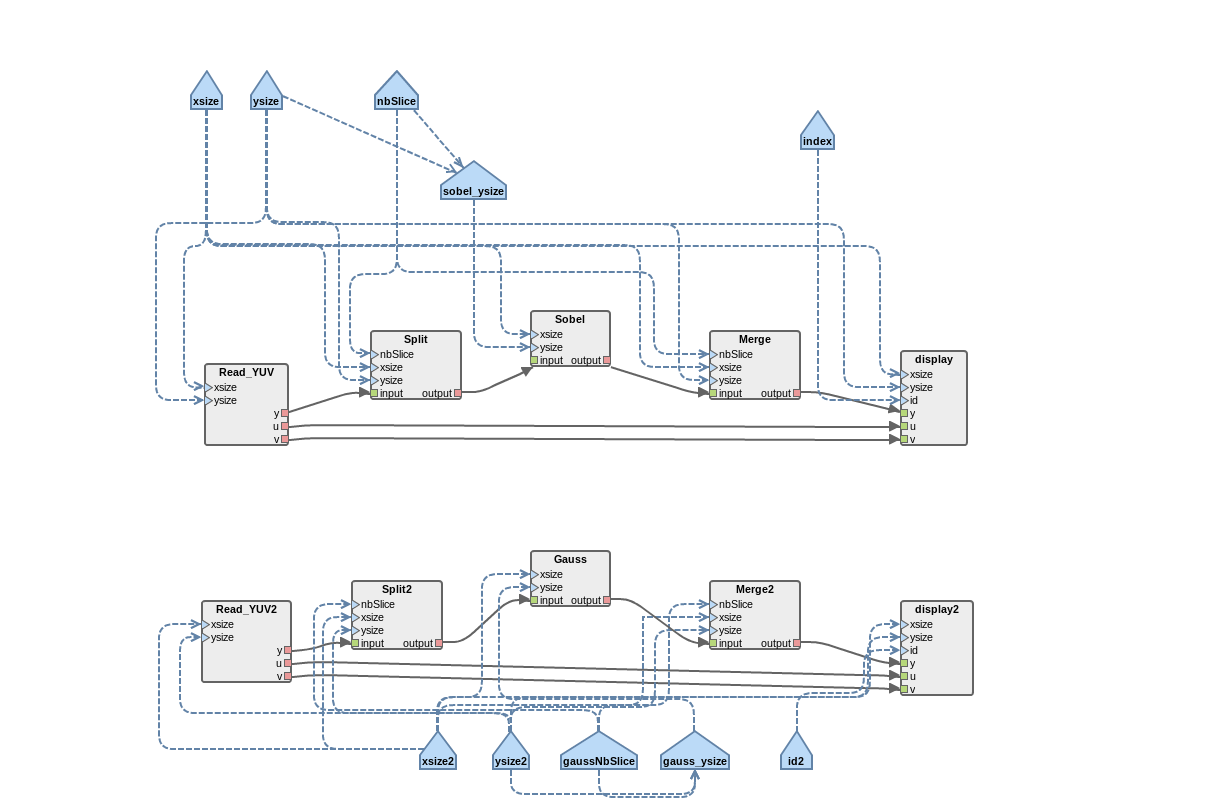
\includegraphics[width=0.99\textwidth]{images/preesm_diagram.png}
    \caption{The PiSDF graph of the PREESM filter application} \end{center}
\end{figure}

To keep the model simple and the program well analyzable both of the processing
paths in the network are independent.

The first actor on both of the processing paths loads the video frames from
memory and passes them to splitting actors. The splitting actor splits the
frames to a suitable number of splices to enable processing of the same video
stream on multiple cores. The filter actor follows the splitting actor. Partial
frames filtered in the filter actor are merged back to whole frames in the merge
actors. The last actors on both of the processing paths are dummy actors.\\

TODO: explain scheduling

\section{OpenEM Filter Application}
The OpenEM implementation of the filter application was heavily influenced by
the PREESM filter application described in \ref{sec:preesmapp}. Specifically the
OpenEM application has to process the frames in similar manner so that only the
scheduling policies between the two programming models should differ. The PREESM
application splits the frames into slices and processes the slices separately
before merging them back into one frame. Similar fork-join mechanism was
implemented in the OpenEM application. Event groups were first planned to be
used as the fork-join mechanism in the filter application but in the final
implementation a different, simpler mechanism was used.

The TI implementation of event groups lacks \texttt{em\_event\_group\_delete}
function which makes it necessary to reuse the existing event groups. The
example applications which are included in the NSN OpenEM distribution
described in \ref{sec:emframework} demonstrate reuse of event groups, but it
was estimated that the programming overhead resulting from the reuse of the
groups would be larger than implementing the fork-join in a simpler manner.

In the final implementation the frames are accumulated simply in a merge buffer
located in shared memory which is referenced through queue context pointers. The
book keeping for frame completion is handled in the same location. The cache
coherency for the book keeping was handled by marking the memory area the merge
buffer resides in as non-cacheable.

\section{PSE Model of OpenEM Filter Application}
\section{Instrumentation}

\chapter{Experiment Results and Analysis}
\label{chapter:results-and-analysis}

\section{Results}
\label{sec:results}
\fixme{Results and discussion on results are both kind of formless blobs of text commenting on mixed findings from the experiments. calls for better division of topics and more structure.}

In this subsection first the results of the measurements of the OpenEM and PREESM applications are presented and next the results of measuring the OpenEM application limited with core masks are presented. The latency and throughput of the OpenEM application measurements are summarized in the tables \ref{tab:oemthrough} and \ref{tab:oemthrough2}. The corresponding summaries for the PREESM application are presented in the table \ref{tab:preesmthrough} The summary of latency and throughtput of the OpenEM application with limited number of cores is presented in table \ref{tab:oemcoremasks}.

The latency of both of the filters is measured from the time the frame is loaded from the memory to the time the frame is merged after filtering. The throughput is measured as frames per second processed in total by the application. Since both of the applications process frames at the same rate from both streams, there is only one FPS measurement for each of the measurement setups. \fixme{maybe move this to construction chapter?}

The latencies of the two streams of the PREESM application in all measurement setups in the table \ref{tab:preesmthrough} are similar. The largest difference in the latencies is in the case where sobel filter filters a CIF stream and gauss filter filters a 4CIF stream, where gauss latency is 60\% higher than the sobel latency. Much larger differences in the latencies are observed with the OpenEM application with two initial events presented in table \ref{tab:oemthrough2} where the largest difference in latencies is also measured between the CIF sobel stream and 4CIF gauss stream. The gauss latency in the particular OpenEM measurement is 200\% higher than the sobel latency. The other OpenEM measurements show larger differences as well compared to PREESM.

\newcommand{\head}[2]{\multicolumn{1}{>{\centering\arraybackslash}p{#1}}{#2}}
\begin{table}
    \begin{center}
        \begin{tabular}{ c c c c c }
            \head{1.5cm}{Sobel latency} & \head{1.5cm}{Gauss latency} &
            \head{1.5cm}{FPS} & \head{1.5cm}{Sobel frame} &
            \head{1.5cm}{Gauss frame} \\ \hline
            5,41 & 8,78 & 223 & CIF & 4CIF \\ \hline
            4,65 & 3,54 & 334 & 4CIF & CIF \\ \hline
            2,15 & 2,51 & 668 & CIF & CIF \\ \hline
            0,61 & 0,71 & 2004 & QCIF & QCIF \\ \hline
        \end{tabular}
        \caption{PREESM latency and throughput. The the latencies are measured in milliseconds.}
        \label{tab:preesmthrough}
    \end{center}
\end{table}
\begin{table}
    \begin{center}
        \begin{tabular}{ c c c c c }
            \head{1.5cm}{Sobel latency} & \head{1.5cm}{Gauss latency} &
            \head{1.5cm}{FPS} & \head{1.5cm}{Sobel frame} &
            \head{1.5cm}{Gauss frame} \\ \hline
            3,59 & 10,93 & 256 & CIF & 4CIF \\ \hline
            3,75 & 2,95 & 527 & 4CIF & CIF \\ \hline
            1,42 & 2,80 & 889 & CIF & CIF \\ \hline
            0,32 & 0,71 & 3534 & QCIF & QCIF \\ \hline
        \end{tabular}
        \caption{OpenEM latency and throughput with 2 frames processed simultaneously. The latencies are measured in milliseconds.}
        \label{tab:oemthrough2}
    \end{center}
\end{table}
\begin{table}
    \begin{center}
        \begin{tabular}{ c c c c c }
            \head{1.5cm}{Sobel latency} & \head{1.5cm}{Gauss latency} &
            \head{1.5cm}{FPS} & \head{1.5cm}{Sobel frame} &
            \head{1.5cm}{Gauss frame} \\ \hline
            15,82 & 22,85 & 599 & CIF & 4CIF \\ \hline
            4,85 & 3,67 & 895 & 4CIF & CIF \\ \hline
            4,91 & 5,96 & 1955 & CIF & CIF \\ \hline
            1,33 & 1,62 & 7819 & QCIF & QCIF \\ \hline
        \end{tabular}
        \caption{OpenEM latency and throughput with 16 frames processed simultaneously. The latencies are measured in milliseconds.}
        \label{tab:oemthrough}
    \end{center}
\end{table}

The PREESM latencies in the table \ref{tab:preesmthrough} are consistently smaller than the latencies of the throughput optimized OpenEM application in the table \ref{tab:oemthrough}. The throughput versus latency balance in the OpenEM application is controlled through the number of frames processed simultaneously.  In this set of measurements the OpenEM application is configured to process 16 frames simultaneously to maximize throughput. \fixme{why is this discussed only here? how about moving this info to construction?} The effect of increasing the number of simultaneous frames was examined by measuring the application with two CIF streams using 2 to 24 initial events. The results of the measurements are presented in table \ref{tab:oeminitialframes}. The latencies get worse and the throughput gets better when the number of frames processed simultaneously increases. This behavior is visualized in figures \ref{fig:oeminitialframesfps} and \ref{fig:oeminitialframeslat}. The throughput grows rapidly up to 8 simultaneous frames after which the growth slows down. The latencies grow with each added frame steadily.

\begin{figure}
    \centering
    \begin{subfigure}[t]{0.49\textwidth}
        \centering
        \includegraphics[width=0.99\linewidth]{images/simultaneous_frames_fps.eps}
        \caption{FPS as a function of simultaneous frames.}
        \label{fig:oeminitialframesfps}
    \end{subfigure}
    \begin{subfigure}[t]{0.49\textwidth}
        \centering
        \includegraphics[width=0.99\linewidth]{images/simultaneous_frames_latency.eps}
        \caption{Latencies as functions of simultaneous frames. The latencies are measured in millisecods.}
        \label{fig:oeminitialframeslat}
    \end{subfigure}
    \caption{The effect of increasing the number of frames processed simultaneously is presented in the figures. The throughput increases rapdily up to 8 simultaneous frames after which the growth slows down. The latency grows more steadily across all measured setups.}
\end{figure}

The throughput of the application is determined by how much time the application spends processing the streams versus the time spent doing something else. For example the synchronization of all cores before each repetition of the PREESM schedule consumes a lot of cpu cycles as is readily observed from the figure \ref{fig:preesmcif}. The portion of the bars marked as busy corresponds to the cycles spent in the synchronization between the repetitions of the schedule. The percentage of cycles spent in the synchronization varies from 16\% on Core 7 to 45\% on Core 0. The OpenEM dynamic scheduler seems to spread out the work more evenly in this case where the total overhead cycles are approximately 60\% for all cores. The core utilization per function is presented in figure \ref{fig:oem8corefunc}. Most of the overhead cycles in the OpenEM application are spent waiting for more frames for processing.

\begin{figure}
    \centering
    \begin{subfigure}[t]{0.49\textwidth}
        \centering
        \includegraphics[width=0.99\linewidth]{images/preesm_cifcif.eps}
        \caption{PREESM}
        \label{fig:preesmcif}
    \end{subfigure}
    \begin{subfigure}[t]{0.49\textwidth}
        \centering
        \includegraphics[width=0.99\linewidth]{images/openem_cifcif_2initial_func.eps}
        \caption{OpenEM}
        \label{fig:oem8corefunc}
    \end{subfigure}
    \caption{In the PREESM graph the busy portion of the bars correspond to the cycles spent synchronizing the cores between the repetitions of the block schedule. The overhead corresponds to cycles spent outside the measured functions and the synchronization. In the OpenEM application the overhead cycles are the cycles spent outside the compared functions.}
\end{figure}

The overhead portions in the figures \ref{fig:preesmcif} and \ref{fig:oem8corefunc} contain all of the data copying from buffer to buffer outside the measured functions, but they also contain different amounts of cycles spent in communications between the cores. The measured functions are the functions which are explicitly called in the PREESM actor model. Other functions not included in the measured functions contain runtime specific communication and some copying of buffers.

\begin{table}
    \begin{center}
        \begin{tabular}{ c c c c }
            \head{1.5cm}{Sobel latency} & \head{1.5cm}{Gauss latency} &
            \head{1.5cm}{FPS} & \head{1.5cm}{Number of cores} \\
            \hline
            57,05 & 57,11 & 263 & 1 \\ \hline
            22,59 & 23,15 & 510 & 2 \\ \hline
            15,09 & 15,84 & 768 & 3 \\ \hline
            10,91 & 11,85 & 1014 & 4 \\ \hline
            8,41 & 9,53 & 1268 & 5 \\ \hline
            7,05 & 8,07 & 1500 & 6 \\ \hline
            5,74 & 6,83 & 1731 & 7 \\ \hline
            4,91 & 5,96 & 1955 & 8 \\ \hline
        \end{tabular}
        \caption{OpenEM measurements with number of cores varied}
        \label{tab:oemcoremasks}
    \end{center}
\end{table}

The second part of this experiment was to limit the number of cores available for the OpenEM application. The resulting latencies and throughputs are presented in the table \ref{tab:oemcoremasks}. The increase of the throughput of the OpenEM application is presented in graph \ref{fig:fpsvcores}. The actual FPS measured with eight cores is approximately 90\% of the linear growth.  

\begin{figure}[h!]
    \begin{center}
        \includegraphics[width=0.7\textwidth]{images/coremask_fps.eps}
        \caption{FPS increase as the function of cores vs. linear growth}
        \label{fig:fpsvcores}
    \end{center}
\end{figure}

\begin{table}
    \begin{center}
        \begin{tabular}{ c c c c }
            \head{1.5cm}{Sobel latency} & \head{1.5cm}{Gauss latency} &
            \head{1.5cm}{FPS} & \head{1.5cm}{Simultaneous Frames} \\
            \hline
            1,42  &  2,80  &  889   &  2 \\ \hline
            1,72  &  3,22  &  1371  &  4 \\ \hline
            2,26  &  3,59  &  1655  &  6 \\ \hline
            2,67  &  3,96  &  1825  &  8 \\ \hline
            3,13  &  4,37  &  1880  &  10 \\ \hline
            3,68  &  4,89  &  1921  &  12 \\ \hline
            4,27  &  5,40  &  1940  &  14 \\ \hline
            4,73  &  5,88  &  1958  &  16 \\ \hline
            5,43  &  6,52  &  1976  &  18 \\ \hline
            6,22  &  7,21  &  1983  &  20 \\ \hline
            6,83  &  7,80  &  1981  &  22 \\ \hline
            7,41  &  8,45  &  1992  &  24 \\ \hline
        \end{tabular}
        \caption{OpenEM measurements with different numbers of frames in processed simultaneously.}
        \label{tab:oeminitialframes}
    \end{center}
\end{table}


\section{Discussion}
\label{sec:discussion}
Three experiments were conducted to understand the performance of OpenEM in stream processing. Stream processing application was implemented with OpenEM and a comparable application was implemented using PREESM. The performance of the application as a part of a stream processing system was not studied. Therefore IO was omitted from the stream processing task that both of the applications implemented.  The experiments focused on understanding the performance of the OpenEM scheduler in handling stream processing tasks.

In this section the results of the three conducted experiments are discussed. First the discoveries made from the experiments are described in \ref{subsec:discoveries}. Second the possible directions of future work are discussed in \ref{subsec:future-work}. Finally the challenges faced conducting the experiments are explained in \ref{subsec:challenges}


\subsection{Discoveries}
\label{subsec:discoveries}
\FloatBarrier
By conducting the three experiments described in this chapter the performance of OpenEM in stream processing was investigated. The first experiment where the throughput and latency of OpenEM were compared to those of PREESM showed that the runtime systems are roughly comparable. This suggests that the dynamic scheduler of OpenEM utilizes the hardware resources efficiently and causes relatively small overhead.

In the second experiment the adaptivity of the OpenEM scheduler was investigated. The second experiment where the number of simultaneously processed frames was varied suggested that by configuring the application the balance between throughput and latency can be controlled. The extent of control the application designer has depends on the complexity of the application. The application measured in the experiments was simple and it is possible that the results overemphasize the adaptivity compared to more complex applications.

The third experiment was conducted to understand the performance improvement gained from making more processing units available for the runtime. The FPS improvement from one to eight cores is close to 90\% of linear improvement, which would suggest the overhead of the scheduler is very small. Since two frames are processed simultaneously the execution of the serial part of the program performed in the read and merge execution objects is interleaved with the execution of the filter execution object of the other frame. This behavior seems to yield a large latency decrease from execution on one core to execution on two cores. Unfortunately this complicates the analysis, since the proportion of the serial and parallel parts of the program is ambiguous. This complication prevents useful comparisons with the theoretical improvement defined by Amdahl's law~\cite{amdahl1967validity}
\begin{figure}
    \centering
    \begin{subfigure}[t]{0.49\textwidth}
        \centering
        \includegraphics[width=0.99\linewidth]{images/openem_cifcif_8cores_eo.eps}
        \caption{Sobel CIF, Gauss CIF}
        \label{fig:oem8coreeo}
    \end{subfigure}
    \begin{subfigure}[t]{0.49\textwidth}
        \centering
        \includegraphics[width=0.99\linewidth]{images/openem_sobel4cif_gausscif_eo.eps}
        \caption{Sobel 4CIF, Gauss Cif}
        \label{fig:oem8coreeosobel4cif}
    \end{subfigure}
    \caption{The bottleneck forming due to the atomic read operation can be observed by comparing the core utilization when both of the streams are at CIF resolution to the case where sobel resolution is increased to 4CIF. In these graphs the application is processing 16 simultaneous events.}
\end{figure}
The throughput optimized application processing 16 events simultaneously exhibits formation of a bottleneck in the atomic execution object. In the table \ref{tab:oemthrough} an improvement of latencies is observed when the workload is made heavier by moving 4CIF stream from gauss filter to the sobel filter while the other stream is kept at CIF resolution.

The probable cause of the improvement of the latencies when the workload is made heavier by increasing the sobel stream resolution is the reduced interleaving of the processing of the subsequent frames. The reduction in the interleaving is caused by the read execution object which is only connected to an atomic queue. When the frame size of the sobel stream is increased the read EO starts limiting the throughput of the application. Fewer frames are processed in parallel which decreases the time from reading each individual frame to the completion of that frame.

The formation of the bottleneck can be observed by comparing the core utilization in the figure \ref{fig:oem8coreeo} to the core utilization in the figure \ref{fig:oem8coreeosobel4cif} where seven cores need to wait for the read operations on the Core 2 and the overall overhead is increased. The other cores do not receive any events from the OpenEM scheduler while waiting.

\begin{figure}[h]
    \begin{center}
        \includegraphics[width=0.49\textwidth]{images/openem_sobelcif_gauss4cif_eo.eps}
        \caption{OpenEM cycles spent per execution object for CIF sobel frames
        and 4CIF gauss frames}
        \label{fig:oem8coreeogauss4cif}
    \end{center}
\end{figure}

When the gauss stream is increased to 4CIF and the sobel stream is kept at CIF the bottleneck does not form. This is likely because computing the gaussian filter for the 4CIF frames is consuming approximately 80\% of the cycles on all cores. In this case the read EO only consumes approximately 5\% to 13\% of the cycles on all cores. Compared to the case of two CIF streams, the latencies in this case are increased by factors of approximately 3 and 4 for sobel and gauss correspondingly. The resulting core utilization graph is presented in figure \ref{fig:oem8coreeogauss4cif}.
\FloatBarrier


\subsection{Future Work}
\label{subsec:future-work}

\subsection{Challenges}
\label{subsec:challenges}
PREESM codegen \\
Unimplemented stuff in TI OpenEM \\
Lacking OpenEM documentation


\chapter{Conclusions}
\label{chapter:conclusion}
\fixme{re-write the first paragraphs} \\
\fixme{From suitability to performance} \\
\fixme{Answers to the questions set in the problem statement} \\
This thesis set out to analyse the suitability of the Texas Instruments implementation of the Open Event Machine multicore runtime to stream processing. The results suggest that OpenEM runtime is flexible enough to support the implementation of such applications. Further research is required to understand the overall suitability of multicore DSPs for stream processing.

A video stream processing application inspired by Canny edge detector was designed. The design was implemented using two distinct multicore runtimes. The baseline application was implemented using PREESM, which generates statically scheduled multicore applications based on synchronous dataflow graphs. The main system under study of this thesis was the OpenEM implementation of the design. To understand the application behavior both applications were instrumented and their execution was measured. The statically scheduled PREESM application achieved lower latency in most of the conducted measurements but the OpenEM application was shown to be well configurable and able to handle dynamic workloads.

High performance stream processing solutions are in demand in the industry. Exploring the use of DSP for stream processing is interesting because they achieve high ratio of floating point operations to power consumption. As multicore DSPs are not as commonly used for stream processing as for example GPUs, the tools for parallel programming have not converged. Runtime systems such as OpenEM have the potential of becoming the standard tools for parallel programming of DSPs.

% Load the bibliographic references
% ------------------------------------------------------------------
% You can use several .bib files:
% \bibliography{thesis_sources,ietf_sources}
\bibliography{sources}


% Appendices go here
% ------------------------------------------------------------------
% If you do not have appendices, comment out the following lines
%\appendix
%\chapter{First appendix: OpenEM and PREESM comparison}
\label{chapter:first-appendix}

\begin{figure}[h!]
    \begin{center}
        \includegraphics[width=0.99\textwidth]{images/openem_cifcif_8cores_eo.eps}
        \caption{OpenEM cycles spent per execution object for CIF sobel frames and CIF gauss frames}
%        \label{fig:oem8coreeo}
    \end{center}
\end{figure}

\begin{figure}[h!]
    \begin{center}
        \includegraphics[width=0.99\textwidth]{images/openem_cifcif_8cores_func.eps}
        \caption{OpenEM cycles spent per function for CIF sobel frames and CIF gauss frames}
%        \label{fig:oem8corefunc}
    \end{center}
\end{figure}

\begin{figure}[h!]
    \begin{center}
        \includegraphics[width=0.99\textwidth]{images/openem_sobel4cif_gausscif_eo.eps}
        \caption{OpenEM cycles spent per execution object for 4CIF sobel frames and CIF gauss frames}
%        \label{fig:oem8coreeosobel4cif}
    \end{center}
\end{figure}

\begin{figure}[h!]
    \begin{center}
        \includegraphics[width=0.99\textwidth]{images/openem_sobel4cif_gausscif_func.eps}
        \caption{OpenEM cycles spent per function for 4CIF sobel frames and CIF gauss frames}
        \label{fig:oem8corefuncsobel4cif}
    \end{center}
\end{figure}

\begin{figure}[h!]
    \begin{center}
        \includegraphics[width=0.99\textwidth]{images/openem_sobelcif_gauss4cif_eo.eps}
        \caption{OpenEM cycles spent per execution object for CIF sobel frames and 4CIF gauss frames}
%        \label{fig:oem8coreeogauss4cif}
    \end{center}
\end{figure}

\begin{figure}[h!]
    \begin{center}
        \includegraphics[width=0.99\textwidth]{images/openem_sobelcif_gauss4cif_func.eps}
        \caption{OpenEM cycles spent per function for CIF sobel frames and 4CIF gauss frames}
        \label{fig:oem8corefuncgauss4cif}
    \end{center}
\end{figure}

\begin{figure}[h!]
    \begin{center}
        \includegraphics[width=0.99\textwidth]{images/openem_sobelqcif_gaussqcif_eo.eps}
        \caption{OpenEM cycles spent per execution object for QCIF sobel frames and QCIF gauss frames}
        \label{fig:oem8coreeoqcif}
    \end{center}
\end{figure}

\begin{figure}[h!]
    \begin{center}
        \includegraphics[width=0.99\textwidth]{images/openem_sobelqcif_gaussqcif_func.eps}
        \caption{OpenEM cycles spent per function for CIF sobel frames and 4CIF gauss frames}
        \label{fig:oem8corefuncqcif}
    \end{center}
\end{figure}

\begin{figure}[h!]
    \begin{center}
        \includegraphics[width=0.99\textwidth]{images/preesm_cifcif.eps}
        \caption{PREESM cycles spent per function for CIF sobel frames and CIF gauss frames}
%        \label{fig:preesmcif}
    \end{center}
\end{figure}

\begin{figure}[h!]
    \begin{center}
        \includegraphics[width=0.99\textwidth]{images/preesm_sobel4cif_gausscif.eps}
        \caption{PREESM cycles spent per function for 4CIF sobel frames and CIF gauss frames}
        \label{fig:preesmsobel4cif}
    \end{center}
\end{figure}

\begin{figure}[h!]
    \begin{center}
        \includegraphics[width=0.99\textwidth]{images/preesm_sobelcif_gauss4cif.eps}
        \caption{PREESM cycles spent per function for CIF sobel frames and 4CIF gauss frames}
        \label{fig:preesmgauss4cif}
    \end{center}
\end{figure}

\begin{figure}[h!]
    \begin{center}
        \includegraphics[width=0.99\textwidth]{images/preesm_sobelqcif_gaussqcif.eps}
        \caption{PREESM cycles spent per function for QCIF sobel frames and QCIF gauss frames}
        \label{fig:preesmgauss4cif}
    \end{center}
\end{figure}


\chapter{Second Appendix: OpenEM coremasks}

\begin{figure}[h!]
    \begin{center}
        \includegraphics[width=0.99\textwidth]{images/openem_cifcif_1cores_eo.eps}
        \caption{OpenEM cycles spent per execution object for CIF sobel frames and CIF gauss frames using 1 core.}
        \label{fig:oem1coreeo}
    \end{center}
\end{figure}

\begin{figure}[h!]
    \begin{center}
        \includegraphics[width=0.99\textwidth]{images/openem_cifcif_1cores_func.eps}
        \caption{OpenEM cycles spent per function for CIF sobel frames and CIF gauss frames using 1 core.}
        \label{fig:oem1corefunc}
    \end{center}
\end{figure}


\begin{figure}[h!]
    \begin{center}
        \includegraphics[width=0.99\textwidth]{images/openem_cifcif_2cores_eo.eps}
        \caption{OpenEM cycles spent per execution object for CIF sobel frames and CIF gauss frames using 2 cores.}
        \label{fig:oem2coreeo}
    \end{center}
\end{figure}

\begin{figure}[h!]
    \begin{center}
        \includegraphics[width=0.99\textwidth]{images/openem_cifcif_2cores_func.eps}
        \caption{OpenEM cycles spent per function for CIF sobel frames and CIF gauss frames using 2 cores.}
        \label{fig:oem2corefunc}
    \end{center}
\end{figure}


\begin{figure}[h!]
    \begin{center}
        \includegraphics[width=0.99\textwidth]{images/openem_cifcif_3cores_eo.eps}
        \caption{OpenEM cycles spent per execution object for CIF sobel frames and CIF gauss frames using 3 cores.}
        \label{fig:oem3coreeo}
    \end{center}
\end{figure}

\begin{figure}[h!]
    \begin{center}
        \includegraphics[width=0.99\textwidth]{images/openem_cifcif_3cores_func.eps}
        \caption{OpenEM cycles spent per function for CIF sobel frames and CIF gauss frames using 3 cores.}
        \label{fig:oem3corefunc}
    \end{center}
\end{figure}


\begin{figure}[h!]
    \begin{center}
        \includegraphics[width=0.99\textwidth]{images/openem_cifcif_4cores_eo.eps}
        \caption{OpenEM cycles spent per execution object for CIF sobel frames and CIF gauss frames using 4 cores.}
        \label{fig:oem4coreeo}
    \end{center}
\end{figure}

\begin{figure}[h!]
    \begin{center}
        \includegraphics[width=0.99\textwidth]{images/openem_cifcif_4cores_func.eps}
        \caption{OpenEM cycles spent per function for CIF sobel frames and CIF gauss frames using 4 cores.}
        \label{fig:oem3corefunc}
    \end{center}
\end{figure}


\begin{figure}[h!]
    \begin{center}
        \includegraphics[width=0.99\textwidth]{images/openem_cifcif_5cores_eo.eps}
        \caption{OpenEM cycles spent per execution object for CIF sobel frames and CIF gauss frames using 5 cores.}
        \label{fig:oem5coreeo}
    \end{center}
\end{figure}

\begin{figure}[h!]
    \begin{center}
        \includegraphics[width=0.99\textwidth]{images/openem_cifcif_5cores_func.eps}
        \caption{OpenEM cycles spent per function for CIF sobel frames and CIF gauss frames using 5 cores.}
        \label{fig:oem5corefunc}
    \end{center}
\end{figure}


\begin{figure}[h!]
    \begin{center}
        \includegraphics[width=0.99\textwidth]{images/openem_cifcif_6cores_eo.eps}
        \caption{OpenEM cycles spent per execution object for CIF sobel frames and CIF gauss frames using 6 cores.}
        \label{fig:oem6coreeo}
    \end{center}
\end{figure}

\begin{figure}[h!]
    \begin{center}
        \includegraphics[width=0.99\textwidth]{images/openem_cifcif_6cores_func.eps}
        \caption{OpenEM cycles spent per function for CIF sobel frames and CIF gauss frames using 6 cores.}
        \label{fig:oem2corefunc}
    \end{center}
\end{figure}

\begin{figure}[h!]
    \begin{center}
        \includegraphics[width=0.99\textwidth]{images/openem_cifcif_7cores_eo.eps}
        \caption{OpenEM cycles spent per execution object for CIF sobel frames and CIF gauss frames using 7 cores.}
        \label{fig:oem7coreeo}
    \end{center}
\end{figure}

\begin{figure}[h!]
    \begin{center}
        \includegraphics[width=0.99\textwidth]{images/openem_cifcif_7cores_func.eps}
        \caption{OpenEM cycles spent per function for CIF sobel frames and CIF gauss frames using 7 cores.}
        \label{fig:oem7corefunc}
    \end{center}
\end{figure}

\begin{figure}[h!]
    \begin{center}
        \includegraphics[width=0.99\textwidth]{images/openem_cifcif_8cores_eo.eps}
        \caption{OpenEM cycles spent per execution object for CIF sobel frames and CIF gauss frames using 8 cores.}
        \label{fig:oem8coreeo2}
    \end{center}
\end{figure}

\begin{figure}[h!]
    \begin{center}
        \includegraphics[width=0.99\textwidth]{images/openem_cifcif_8cores_func.eps}
        \caption{OpenEM cycles spent per function for CIF sobel frames and CIF gauss frames using 8 cores.}
        \label{fig:oem8corefunc2}
    \end{center}
\end{figure}

\begin{figure}[h!]
    \begin{center}
        \includegraphics[width=0.99\textwidth]{images/coremask_fps.eps}
        \caption{FPS increase as the function of cores vs. linear growth}
%        \label{fig:fpsvcores}
    \end{center}
\end{figure}

\begin{figure}[h!]
    \begin{center}
        \includegraphics[width=0.99\textwidth]{images/coremask_latencies.eps}
        \caption{Latency decrease as the function of cores}
        \label{fig:latencyvcores}
    \end{center}
\end{figure}


% End of document!
% ------------------------------------------------------------------
% The LastPage package automatically places a label on the last page.
% That works better than placing a label here manually, because the
% label might not go to the actual last page, if LaTeX needs to place
% floats (that is, figures, tables, and such) to the end of the
% document.
\end{document}
